\section{Resultados}
\label{sec:resultados}

\subsection{Caracterização do Conjunto de Dados}

Nesta subseção sintetizamos as principais características do conjunto utilizado na calibração. Após o tratamento de valores ausentes, o dataset contém 9\,471 observações horárias compreendendo o período de 2004--2005, com medições concomitantes de sensores MOx, variáveis meteorológicas e poluentes de referência. Destaca-se a presença de forte assimetria em variáveis como NOx(GT), NMHC(GT) e CO(GT), bem como uma assimetria moderada no alvo NO$_2$, o que justifica o uso de transformações logarítmicas e padronização antes do ajuste dos modelos.

Os sensores PT08.* capturam respostas elétricas sensíveis a diferentes espécies (CO, compostos orgânicos voláteis, NOx, NO$_2$ e O$_3$), enquanto T, RH e AH caracterizam o estado termodinâmico do ambiente. Essa combinação oferece um cenário típico de calibração de sensores de baixo custo, no qual multicolinearidade e correlações espúrias entre condições meteorológicas e concentração de poluentes são a regra.

\subsection{Análise Exploratória}

As análises exploratórias visam compreender o comportamento temporal do NO$_2$, a presença de sazonalidade e a distribuição das variáveis preditoras, elementos que influenciam diretamente a escolha de modelos e estratégias de pré-processamento.

\begin{figure}[h]
\centering
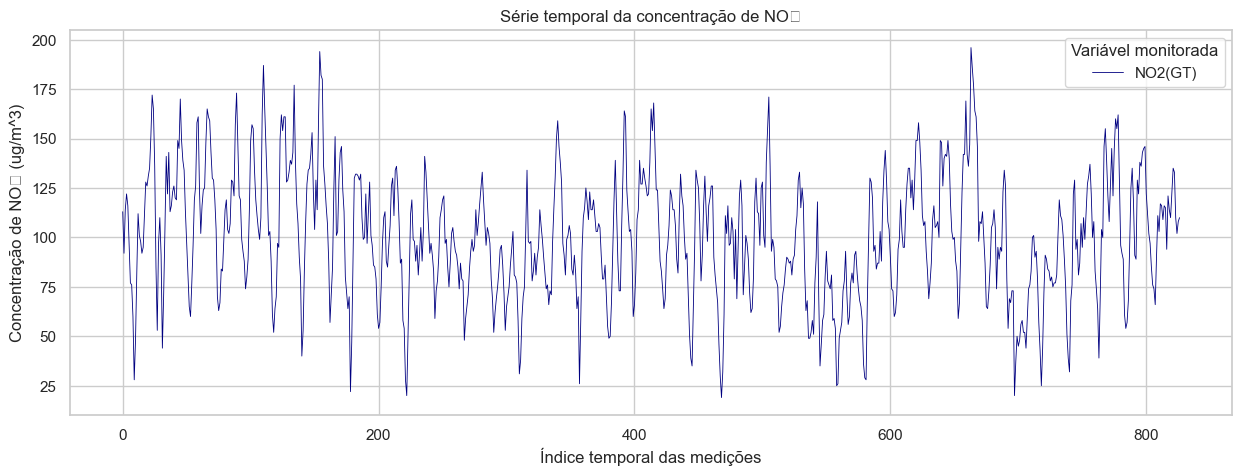
\includegraphics[width=\columnwidth]{figures/eda_temporal_behavior.png}
\caption{Série temporal da concentração de NO$_2$}
\label{fig:eda_temporal_behavior}
\end{figure}

A Figura~\ref{fig:eda_temporal_behavior} mostra a série temporal de NO2(GT) ao longo do período monitorado. Observam-se flutuações acentuadas, com episódios de alta concentração intercalados com períodos de menor carga, sugerindo influência combinada de padrões de emissão (tráfego, atividades urbanas) e condições meteorológicas. A ausência de tendência monótona reforça a necessidade de modelos que capturem relações instantâneas entre sensores e referência, mais do que uma dinâmica temporal complexa.

\begin{figure}[h]
\centering
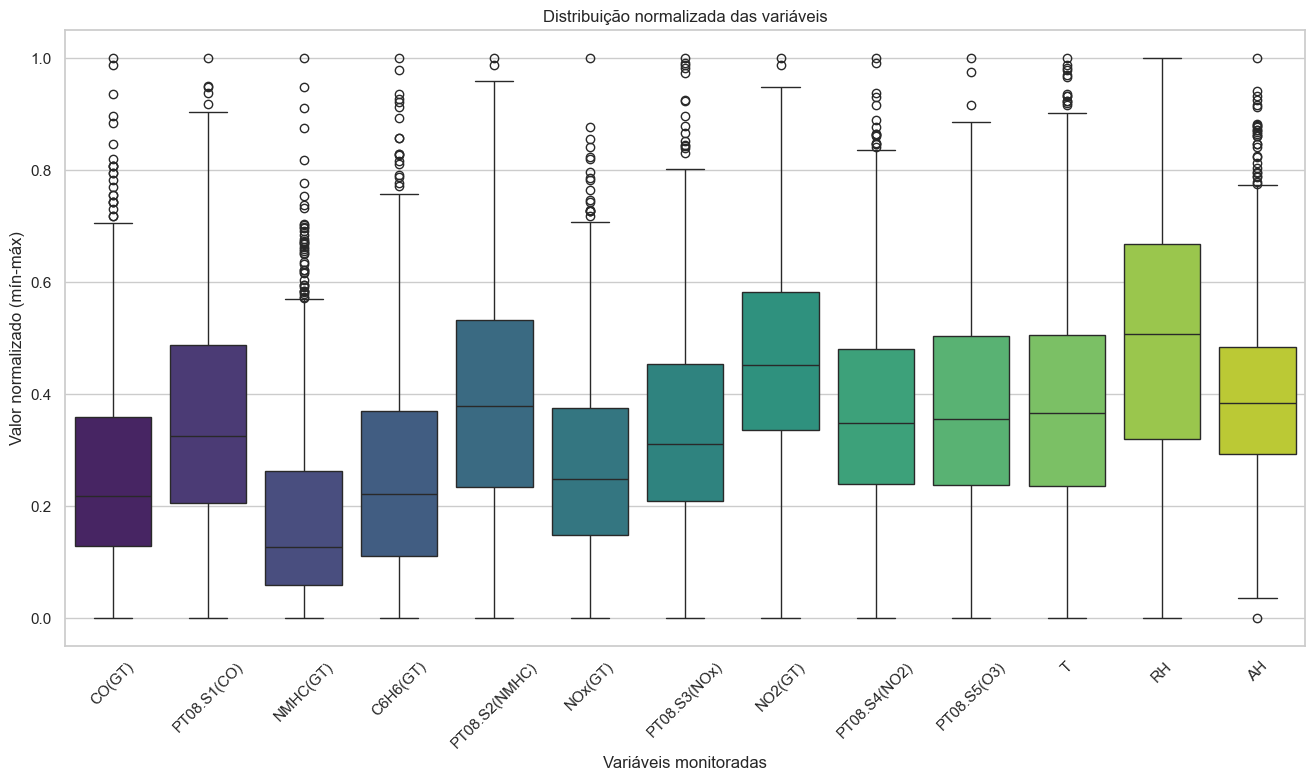
\includegraphics[width=\columnwidth]{figures/eda_boxplots_outliers.png}
\caption{Distribuição normalizada das variáveis}
\label{fig:eda_boxplots_outliers}
\end{figure}

A Figura~\ref{fig:eda_boxplots_outliers}, construída a partir de variáveis normalizadas, evidencia a presença de caudas longas e possíveis outliers em variáveis como NOx(GT), NMHC(GT) e CO(GT), bem como assimetrias em algumas respostas dos sensores MOx. Esse padrão indica que uma parcela reduzida de observações concentra valores muito altos, o que pode distorcer ajustes puramente lineares sem tratamento prévio.

% Figura de histograma removida conforme orientação

\begin{figure}[h]
\centering
\IfFileExists{figures/eda_correlation_heatmap.png}{%
	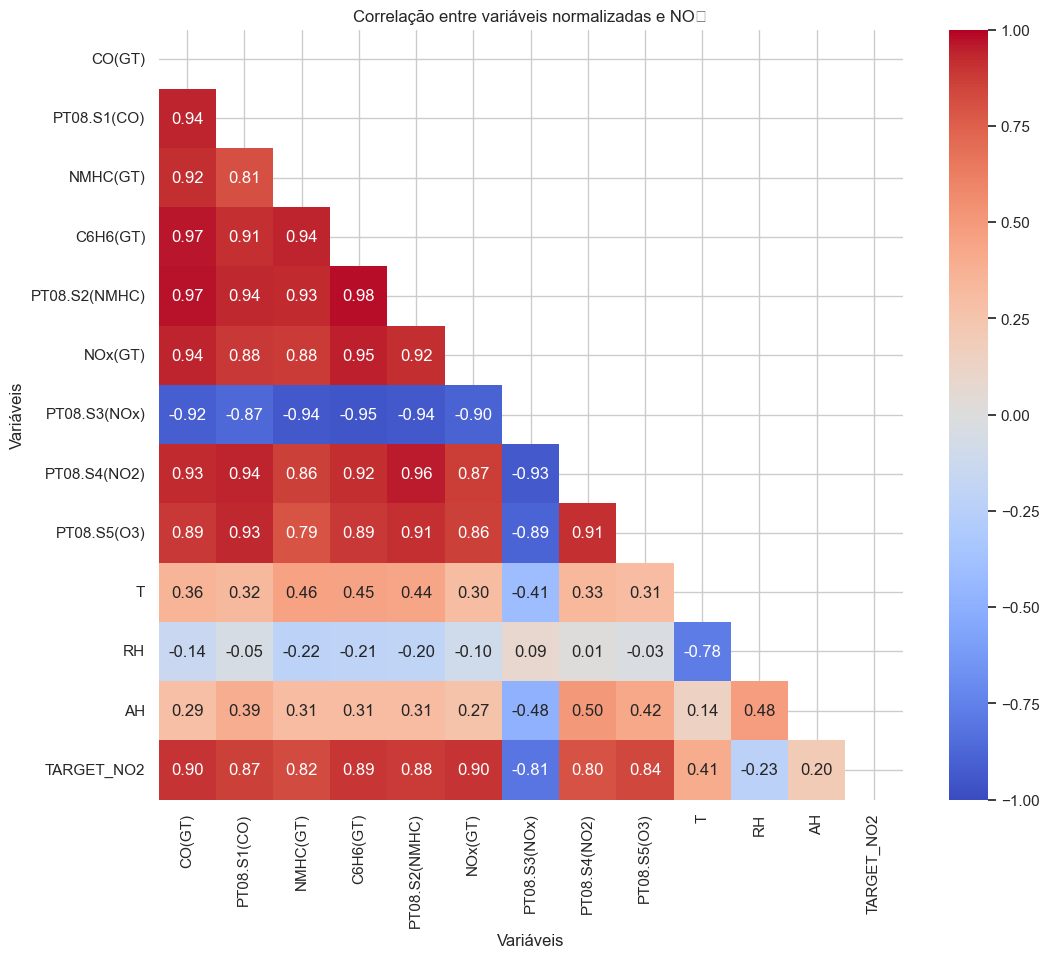
\includegraphics[width=\columnwidth]{figures/eda_correlation_heatmap.png}%
}{%
	% Figura de correla\c{c}\~ao ainda n\~ao gerada pelo notebook
}
\caption{Matriz de correla\c{c}\~ao entre preditores transformados e NO$_2$.}
\label{fig:corr_heatmap}
\end{figure}

A Figura~\ref{fig:corr_heatmap} apresenta a matriz de correla\c{c}\~ao de Pearson entre todos os preditores transformados e o alvo NO$_2$. Observa-se um bloco de correla\c{c}\~oes elevadas entre vari\'aveis relacionadas a NO$_x$/NO$_2$ (por exemplo, NOx(GT), PT08.S3(NOx) e PT08.S4(NO2)), bem como correla\c{c}\~oes moderadas com algumas vari\'aveis meteorol\'ogicas. Esse padr\~ao confirma a presen\c{c}a de multicolinearidade e motiva o uso de modelos regularizados (Ridge) e baseados em componentes supervisionados (PLS).

\subsection{Modelos de Regressão}

\subsubsection{Regressão Linear Ordinária (OLS)}

\begin{figure}[h]
\centering
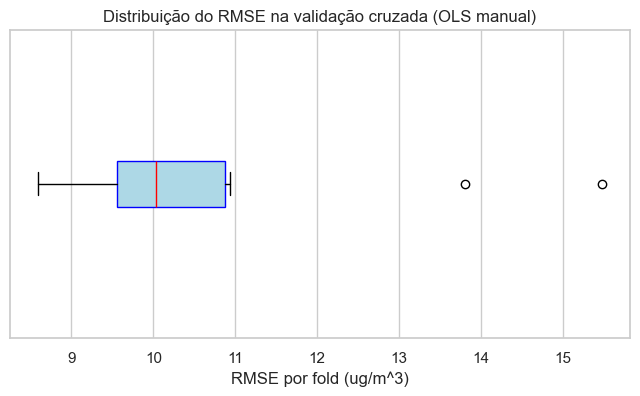
\includegraphics[width=\columnwidth]{figures/ols_cv_boxplot.png}
\caption{Distribuição do RMSE na validação cruzada (OLS manual)}
\label{fig:ols_cv_boxplot}
\end{figure}

A Figura~\ref{fig:ols_cv_boxplot} resume a distribuição do RMSE ao longo dos 10 folds de validação cruzada. A variabilidade moderada entre folds indica que o desempenho do modelo é relativamente sensível à composição do conjunto de treino, fenômeno esperado em cenários com multicolinearidade e ausência de regularização explícita.

\subsubsection{Regressão Ridge}

\begin{table}[t]
  \centering
  \caption{Ridge: comparação entre implementação manual e \textit{scikit-learn}}
  \label{tab:resultados_ridge}
\begin{tabular}{lrrrrr}
Modelo & $\lambda$ & $RMSE_\text{teste}$ & $R^{2}_\text{teste}$ & $RMSE_\text{CV}$ & $R^{2}_\text{CV}$ \\
Manual & 2.154435 & 10.464948 & 0.895018 & 10.567846 & 0.880259 \\
Sklearn & 2.154435 & 10.464948 & 0.895018 & 10.756799 & 0.877137 \\
\end{tabular}

\end{table}


\begin{figure}[h]
\centering
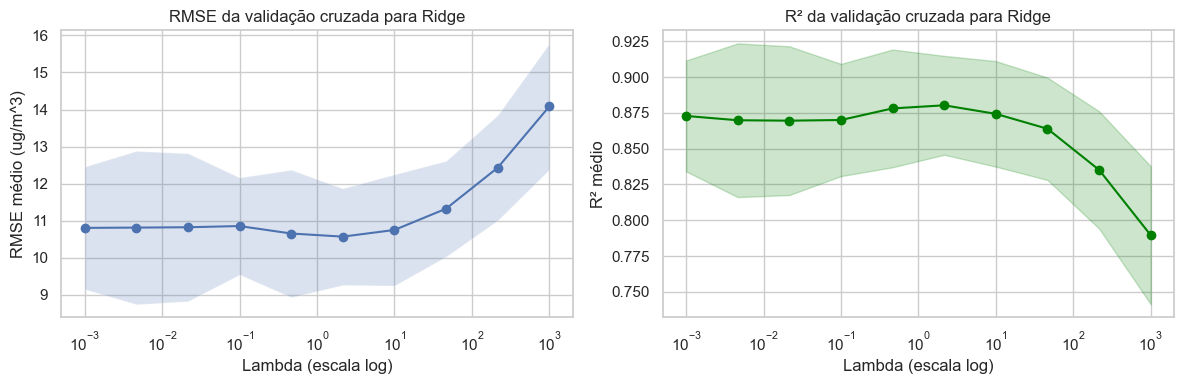
\includegraphics[width=\columnwidth]{figures/ridge_cv_profile.png}
\caption{RMSE e R² da validação cruzada para Ridge}
\label{fig:ridge_cv_profile}
\end{figure}

A regressão Ridge introduz uma penalização L2 sobre os coeficientes, mitigando problemas de multicolinearidade. A Tabela~\ref{tab:resultados_ridge} mostra que o melhor valor de $\lambda$ encontrado (aprox. 2{,}15) produz RMSE de teste em torno de 10{,}46 e $R^2$ de 0{,}895, muito próximos aos resultados da implementação do \textit{scikit-learn}, o que valida a implementação manual.

A Figura~\ref{fig:ridge_cv_profile} revela como RMSE e $R^2$ médios em validação cruzada variam com $\lambda$. Para valores muito baixos de penalização, o modelo se aproxima da OLS e apresenta leve instabilidade; à medida que $\lambda$ aumenta até a região ótima, observa-se redução do RMSE médio e maior estabilidade entre folds. Penalizações excessivas, por outro lado, degradam progressivamente o ajuste, como esperado.

\subsubsection{Regressão PLS}

\begin{figure}[h]
\centering
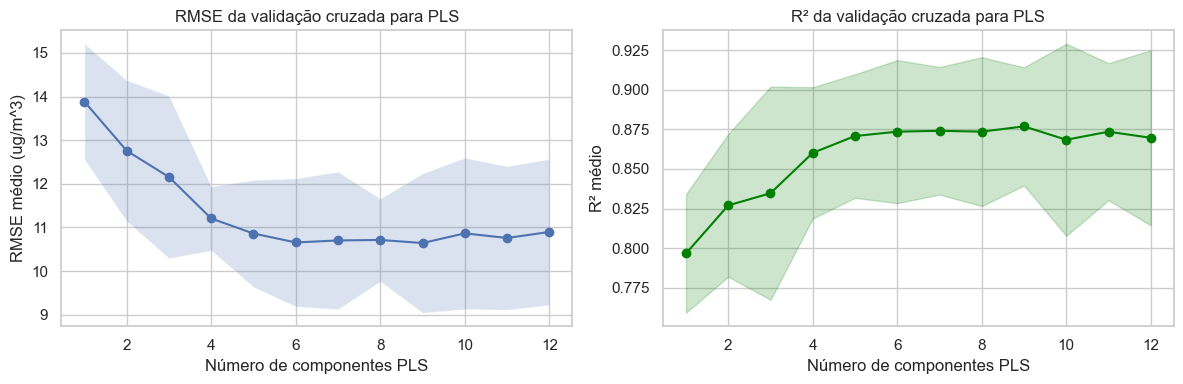
\includegraphics[width=\columnwidth]{figures/pls_cv_profile.png}
\caption{RMSE e R² da validação cruzada para PLS}
\label{fig:pls_cv_profile}
\end{figure}

O PLS busca componentes latentes supervisionados que maximizam a covariância entre preditores e alvo, sendo especialmente adequado em cenários com muitas variáveis correlacionadas. O melhor modelo selecionado pela validação cruzada utiliza 9 componentes, alcançando RMSE de teste de aproximadamente 10{,}44 e $R^2$ de 0{,}895, com valores médios de RMSE e $R^2$ em CV muito próximos aos observados em teste. Esses resultados são equivalentes aos obtidos com Ridge e ligeiramente superiores aos da OLS, reforçando a boa capacidade de generalização do modelo.

\begin{figure}[h]
\centering
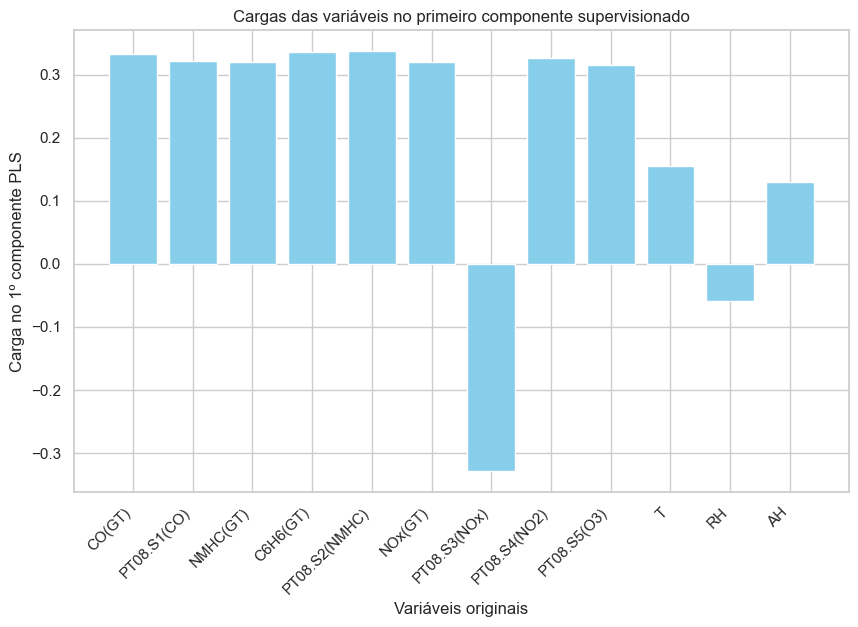
\includegraphics[width=\columnwidth]{figures/pls_loadings.png}
\caption{Cargas das variáveis no primeiro componente PLS}
\label{fig:pls_loadings}
\end{figure}

A Figura~\ref{fig:pls_cv_profile} mostra que o RMSE médio em validação cruzada diminui rapidamente com o aumento do número de componentes até a vizinhança de 9, estabilizando-se a partir daí. A Figura~\ref{fig:pls_loadings} sugere que poucas combinações de preditores dominam a direção supervisionada, reforçando a utilidade de componentes latentes em presença de multicolinearidade. Os gráficos de valores observados versus previstos (não mostrados) apresentam padrão semelhante ao obtido com Ridge, coerente com os indicadores numéricos.

\subsubsection{Rede Neural MLP}

\begin{table}[t]
  \centering
  \caption{Resultados do Modelo MLP}
  \label{tab:resultados_mlp}
\begin{tabular}{lrr}
Modelo & RMSE Teste & R2 Teste \\
OLS Sklearn & 10.403632 & 0.896244 \\
MLP (1 hidden) & 13.217788 & 0.832521 \\
Ridge Sklearn & 10.464948 & 0.895018 \\
PLS (best CV) & 10.441786 & 0.895482 \\
\end{tabular}

\end{table}

A rede neural MLP com uma camada oculta de 64 neurônios foi adotada como referência não linear. A Tabela~\ref{tab:resultados_mlp} mostra que, nesta configuração, o MLP apresenta RMSE de teste em torno de 13{,}2 e $R^2$ de aproximadamente 0{,}83, significativamente piores que os modelos lineares, com maior espalhamento em torno da reta ideal.

Esse resultado sugere que, para o tamanho de amostra disponível e o pré-processamento adotado, a complexidade adicional do MLP não se traduz em ganho de desempenho, possivelmente devido à necessidade de ajuste mais cuidadoso de arquitetura, regularização e taxa de aprendizado.

\subsection{Comparação de Desempenho}

A Tabela~\ref{tab:desempenho_modelos} sintetiza o desempenho dos quatro modelos em termos de RMSE e $R^2$ médios na validação cruzada e no conjunto de teste. Em linhas gerais, OLS, Ridge e PLS apresentam RMSE de teste na faixa de 10{,}4--10{,}8 e $R^2$ entre 0{,}87 e 0{,}90, indicando ajuste consistente e relativamente estável.

Ridge e PLS exibem leve vantagem em termos de estabilidade em validação cruzada e desempenho médio, refletindo a capacidade de lidar com multicolinearidade (via penalização L2 ou componentes supervisionados). O MLP, por sua vez, apresenta RMSE e variabilidade consideravelmente maiores, com $R^2$ inferior, sinalizando que, neste cenário específico, a complexidade não linear não se traduz em melhor poder preditivo.

\begin{table}[t]
  \centering
  \caption{Desempenho dos Modelos}
  \label{tab:desempenho_modelos}
\begin{tabular}{lrrrr}
Modelo & $RMSE_\text{CV}$ & $R^{2}_\text{CV}$ & $RMSE_\text{teste}$ & $R^{2}_\text{teste}$ \\
OLS & 10.931799 & 0.872322 & 10.403632 & 0.896244 \\
Ridge & 10.756799 & 0.877137 & 10.464948 & 0.895018 \\
PLS & 10.642892 & 0.876887 & 10.441786 & 0.895482 \\
MLP & 13.564981 & 0.805638 & 13.217788 & 0.832521 \\
\end{tabular}

\end{table}

\subsection{Importância das Variáveis}

Por fim, a análise dos coeficientes padronizados estimados pelo modelo Ridge, combinada com os loadings do primeiro componente PLS (Figura~\ref{fig:pls_loadings}), indica que um subconjunto reduzido de preditores tem influência muito maior na calibração do NO$_2$ do que o restante. Em particular, variáveis diretamente relacionadas a NOx/NO$_2$ e algumas variáveis meteorológicas exercem papel predominante, enquanto demais preditores têm contribuição marginal.

Em conjunto, esses resultados reforçam que a calibração de sensores de baixo custo para NO$_2$ pode ser conduzida com alto grau de acurácia utilizando modelos lineares bem regularizados e um pré-processamento cuidadoso, sem necessidade de arquiteturas não lineares mais complexas para este conjunto de dados.
